\documentclass{tuftebook}

\usepackage[utf8]{inputenc}
\usepackage[T1]{fontenc}
\usepackage{textcomp}

\usepackage{url}

\usepackage[
    sorting=nyt,
    style=alphabetic
]{biblatex}
\addbibresource{bibliography.bib}

\usepackage{hyperref}
\hypersetup{
    colorlinks,
    linkcolor={black},
    citecolor={black},
    urlcolor={blue!80!black}
}



\newcommand{\highlight}[1]{\textcolor{jade}{#1}}
\newcommand{\vektor}[3]{\begin{pmatrix} #1 \\ #2 \\ #3\end{pmatrix}}
\usepackage{xcolor}
\definecolor{jade}{HTML}{00A36C}
\definecolor{crimson}{HTML}{DC143C}
\definecolor{pinke}{HTML}{FF1493}
\definecolor{babyblau}{HTML}{0096FF}

% Adds Bibliography, ... to Table of Contents
\usepackage[nottoc]{tocbibind}

\usepackage{graphicx}
\usepackage{float}

% \usepackage{cmbright}

\usepackage{mult icol}
\usepackage{pgfplots}
\pgfplotsset{compat=1.18}
\usepackage{amsmath, amsfonts, mathtools, amsthm, amssymb}
\usepackage{mathrsfs}
\usepackage{cancel}

\newcommand\N{\ensuremath{\mathbb{N}}}
\newcommand\R{\ensuremath{\mathbb{R}}}
\newcommand\Z{\ensuremath{\mathbb{Z}}}
\renewcommand\O{\ensuremath{\emptyset}}
\newcommand\Q{\ensuremath{\mathbb{Q}}}
\newcommand\C{\ensuremath{\mathbb{C}}}
\let\implies\Rightarrow
\let\impliedby\Leftarrow
\let\iff\Leftrightarrow
\let\epsilon\varepsilon

\usepackage{tikz}
\usepackage{tikz-cd}

% theorems
\usepackage{thmtools}
\usepackage{thm-restate}
\usepackage[framemethod=TikZ]{mdframed}
\mdfsetup{skipabove=1em,skipbelow=0em, innertopmargin=12pt, innerbottommargin=8pt}

\theoremstyle{definition}

\usepackage{thmtools}
\usepackage{thm-restate}
\usepackage[framemethod=TikZ]{mdframed}
\mdfsetup{skipabove=1em,skipbelow=0em, innertopmargin=12pt, innerbottommargin=8pt}

\theoremstyle{definition}

\makeatletter

\declaretheoremstyle[headfont=\bfseries\sffamily, bodyfont=\normalfont, mdframed={ nobreak }, headpunct={} ]{thmgreenbox}
\declaretheoremstyle[headfont=\bfseries\sffamily, bodyfont=\normalfont, mdframed={ nobreak } ]{thmredbox}
\declaretheoremstyle[headfont=\bfseries\sffamily, bodyfont=\normalfont]{thmbluebox}
\declaretheoremstyle[headfont=\bfseries\sffamily, bodyfont=\normalfont]{thmblueline}
\declaretheoremstyle[headfont=\bfseries\sffamily, bodyfont=\normalfont, numbered=no, mdframed={ rightline=false, topline=false, bottomline=false, }, qed=\qedsymbol ]{thmproofbox}
\declaretheoremstyle[headfont=\bfseries\sffamily, bodyfont=\normalfont, numbered=no, mdframed={ nobreak, rightline=false, topline=false, bottomline=false } ]{thmexplanationbox}

\declaretheoremstyle[headfont=\bfseries\sffamily, bodyfont=\normalfont, numbered=no, mdframed={ nobreak, rightline=false, topline=false, bottomline=false } ]{thmexplanationbox}


\declaretheorem[style=thmgreenbox,numbered=no,name={}]{definition}
\declaretheorem[style=thmredbox,numbered=yes,name={Postulat}]{postulat}
\declaretheorem[style=thmredbox,numbered=no,name={Beobachtung}]{beobachtung}
\declaretheorem[style=thmredbox,numbered=no,name={Deutung}]{deutung}
\declaretheorem[style=thmredbox,numbered=no,name={Erklärung}]{erklaerung}
\declaretheorem[style=thmredbox,numbered=no,name={Schlussfolgerung}]{schlussfolgerung}
\declaretheorem[style=thmredbox,numbered=yes,name={Typ}]{typ}

% \renewenvironment{proof}[1][\proofname]{\begin{replacementproof}}{\end{replacementproof}}

% \AtEndEnvironment{eg}{\null\hfill$\diamond$}%

\newtheorem*{uovt}{UOVT}
\newtheorem*{notation}{Notation}
\newtheorem*{previouslyseen}{As previously seen}
\newtheorem*{problem}{Problem}
\newtheorem*{observe}{Observe}
\newtheorem*{property}{Property}
\newtheorem*{intuition}{Intuition}


\declaretheoremstyle[
    headfont=\bfseries\sffamily\color{RawSienna!70!black}, bodyfont=\normalfont,
    mdframed={
        linewidth=2pt,
        rightline=false, topline=false, bottomline=false,
        linecolor=RawSienna, backgroundcolor=RawSienna!5,
    }
]{todo}
\declaretheorem[numbered=no, style=todo, name=TODO]{TODO}


\usepackage{etoolbox}
\AtEndEnvironment{vb}{\null\hfill$\diamond$}%
\AtEndEnvironment{intermezzo}{\null\hfill$\diamond$}%

% http://tex.stackexchange.com/questions/22119/how-can-i-change-the-spacing-before-theorems-with-amsthm
% \def\thm@space@setup{%
%   \thm@preskip=\parskip \thm@postskip=0pt
% }

\usepackage{xifthen}

\makeatother

% figure support (https://castel.dev/post/lecture-notes-2)
\usepackage{import}
\usepackage{xifthen}
\pdfminorversion=7
\usepackage{pdfpages}
\usepackage{transparent}


\makeatletter
\newif\ifworking
\@ifclasswith{tuftebook}{working}{\workingtrue}{\workingfalse}
\makeatother

\newcommand{\incfig}[2][1]{%
    % \ifworking{\makebox[0pt][c]{\color{gray}{\scriptsize\textsf{#2}}}}\fi%
    \def\svgwidth{#1\textwidth}
    \import{./figures/}{#2.pdf_tex}
}

\newcommand{\fullwidthincfig}[2][0.90]{%
    % \ifworking{\makebox[0pt][l]{\color{gray}{\scriptsize\textsf{#2}}}}\fi%
    \def\svgwidth{#1\paperwidth}
    \import{./figures/}{#2.pdf_tex}
}



\newcommand{\minifig}[2]{%
    \def\svgwidth{#1}%
    \begingroup%
    \setbox0=\hbox{\import{./figures/}{#2.pdf_tex}}%
    \parbox{\wd0}{\box0}\endgroup%
    \hspace*{0.2cm}
}

% %http://tex.stackexchange.com/questions/76273/multiple-pdfs-with-page-group-included-in-a-single-page-warning
\pdfsuppresswarningpagegroup=1

\newcommand\todo[1]{\ifworking {{\color{red}{#1}}} \else {}\fi}
\newcommand\charlotte[1]{\ifworking {{\color{blue}{#1}}} \else {}\fi}

\author{Gilles Castel}



\usepackage{multirow}
\def\block(#1,#2)#3{\multicolumn{#2}{c}{\multirow{#1}{*}{$ #3 $}}}

% \overfullrule=1mm

\newenvironment{myproof}[1][\proofname]{%
  \proof[\rm \bf #1]%
}{\endproof}

\begin{document}


\section{Strahlung und Materie}
    \noindent Gasatome können nur bestimmte und für das Element jeweils charakteristische Energiebeträge aufnehmen bzw. abgeben. Die Energieabgabe geschiecht durch die \highlight{Emission von Photonen}. Das nun verwendete System "Atom" besitzt dementsprechd nur ganz bestimmte Energiezustände. Diese Vorstellung des Atoms resultiert aus dem \highlight{Bohrschen Atommodell}.
    


\subsection{Physik der Atomhülle}
    \subsubsection{Bohr'sches Atommodell}
    \begin{marginfigure}
        \centering
        \def\svgwidth{\linewidth}
        \import{./figures/}{bohratomodell.pdf_tex}
        \caption{Bohr'sches Atommodell}
        \label{fig:bohrmodell}
    \end{marginfigure}
    Das einfachste Atom ist das Wasserstoffatom. Der Atomkern besteht aus einem Proton, die Hülle wird von einenm Elektron gebildet. Das emittierte Licht eines Wasserstoffatoms kann zu Serien zusammengefasst werden. Diese Serien lassen sich erklären, wenn das Wasserstoffatom nur \highlight{diskrete Energienieveaus} $E_n$ besitzt: \[E_n=-13.6\,\text{eV}\cdot\frac{1}{n^2}\quad\text{mit}\quad n=1,2,3,\ldots\]
    Sind das Elektron und das Proton sehr weit voneinander entfernt und werden die beiden einander soweit angenähert, dass ein gebundenes System minimaler Energie entsteht, so wird ein Energiebetrag von $13.6$ eV abgegeben. Das Wasserstoffatom besitzt daher ein Energieniveau, das $13.6$ eV unterhalb der Energie im getrennten Fall liegt.
    Das bedeutet, dass ein Energiebetrag von $13.6$ eV nötig ist, um das Elektron ganz vom Kern zu entfernen (\highlight{ionisieren}). $n=1$ und $n_1=K$ ist somit der Grundzustand, also der Zustand mit dem niedrigsten Energiewert von $13.6$ eV.
    
    \begin{marginfigure}
        \centering
        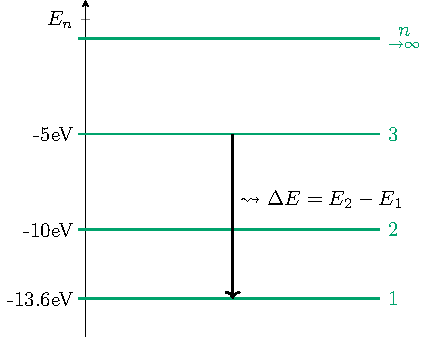
\includegraphics[width=\linewidth]{figures/energieniveaus.pdf}
        \caption{Energieniveauschema}
        \label{fig:energieniveauschema}
    \end{marginfigure}
    Wird dem Atom eine geringere, aber passende Energie zugeführt, so kann es vom Grundzustand in einen höheren, angeregten Zustan ($n=2,3,\ldots$) versetzt werden. Anschaulich werden diese Energieniveaus des Atoms durch die Darstellung in einem \hyperref[fig:energieniveauschema]{Energieniveauschema}, auch \highlight{Term-schema} genannt.
    Hierzu wird auf der vertikalen Achse die Energie aufgetragen. Durch waagerechte Linien werden die diskreten Energiniveaus dargestellt. So wird deutlich, dass zwischen den Linien keine weiteren erlaubten Energiezustände des Atoms existieren. 

    \begin{definition}
        \vspace{-1em}
        Befindet sich ein Atom in einem angeregten Zustand, so besitzt es eine Energie, die größer ist als die des Grundzustandes. Es verbleibt nur eine sehr kurze Zeit (etwa $10^{-8}$s) in diesem Zustand. Durch \highlight{Emission eines Photons} mit der Energie, die gleich der Energiedifferenz ($\leadsto\Delta E$) der beiden Niveaus ist, gelangt das Atom wieder in einen energetisch tieferen Zustand.
    \end{definition}
    Niels Bohr postulierte 1913 das \highlight{Bohrsche Atommodell}, das die Quantisierung der Energiezustände des Atoms beschreibt. Dieses Modell basiert auf folgenden Postulaten:

    \begin{postulat}
        \vspace{-1em}
        (Diskrete Energiestufen):
        \vspace{\baselineskip}
        
        \noindent Die Energie eines Elektrons im Atom kann nur diskrete Werte \highlight{$E_n$} annehmen.
    \end{postulat}
    Werden die diskreten Energiewerte erreicht, so wird das Atom in einen angeregten Zustand versetzt. Die Energiedifferenz zwischen zwei Niveaus ist gleich der Energie des emittierten Photons. Die Energie des Photons ist also quantisiert.

    \begin{postulat}
        \vspace{-1em}
        (Lichtemission):
        \vspace{\baselineskip}

        \noindent Die Frequenz der ausgesendeten elektromagnetischen Strahlung ergibt sich aus der Energiedifferenz zwischen dem Ausgangs- und Endzustand.
        \begin{equation}
            h\cdot f=E_m-E_n\quad\text{mit}\quad m,n\in\mathbb{N}\quad\text{und}\quad m>n
        \label{eq:lichtemission}
        \end{equation}
    \end{postulat}
    Führt ein Elektron einen \highlight{Quantensprung} aus, so wird elektromagnetische Strahlung in Form von Photonen emittiert.

    \begin{marginfigure}
        \centering
        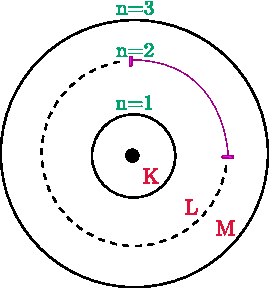
\includegraphics[width=\linewidth]{figures/bohratomodell2.pdf}
        \caption{Grafische Darstellung der Quantenbedingung}
        \label{fig:quantenbedingung}
    \end{marginfigure}
    \begin{postulat}
        \vspace{-1em}
        (Quantenbedingung):
        \vspace{\baselineskip}

        \noindent Der Umlauf der Elektronen erfolgt nur auf bestimmten diskreten Bahnen. Auf diesen Bahnen wird keine Energie abgestrahlt. Die Bahnen müssen die folgende Quantenbedingung erfüllen: 
        \begin{equation}
            m_e\cdot v_n\cdot r_n=\frac{n\cdot h}{2\cdot\pi}
            \label{eq:quantenbedingung}
        \end{equation}
    \end{postulat}
    Die Quantenbedingung beschreibt die Bedingung, die die Bahnen der Elektronen im Atom erfüllen müssen. Die Bahnen sind durch den Bahnradius $r_n$ und die Bahngeschwindigkeit $v_n$ definiert. Die Quantenbedingung stellt sicher, dass die Elektronen nur auf bestimmten Bahnen um den Kern kreisen können. Die Bahnen sind durch die Quantenbedingung quantisiert.



    \subsubsection{Die Quantenhafte Emission und Absorption}
    Wie wir bereits in \hyperref[eq:lichtemission]{dem Postulat für Lichtemission} festgehalten haben, wird bei einem Quantensprung eines Elektrons elektromagnetische Strahlung in Form von Photonen emittiert. Die Energie des Photons ist gleich der Energiedifferenz zwischen den beiden Niveaus. Die Frequenz des Photons ergibt sich aus der Energie des Photons durch die Plancksche Formel:
    \begin{equation}
        E=h\cdot f=h\cdot\frac{c}{\lambda}
        \label{eq:planckf}
    \end{equation}
    Diese Emission wird auch \highlight{Quantenhafte Emission} genannt, da das Elektron nur so viel Energie abgeben kann, wie die Energiedifferenz zwischen den Niveaus beträgt
    \begin{definition}
        \vspace{-1em}
        Natriumatome absoriberen Phtonen genau der Energie und Wellenlänge, die auch von ihnen ausgesendet werden. Dieser spezielle Effekt heißt \highlight{Umkehr der Natriumlinie}.
    \end{definition}
    Der Vorgang, dass ein Atom  durch Absorption eines Photons angeregt wird und bei Rückkehr in den ursprünglichen Zustand ein gleichartiges Photon wieder aussendet, wird als \highlight{Resonanzabsorption} bezeichnet.
    \begin{definition}
        \vspace{-1em}
        Atome können Photonen absorbieren, die die gleiche Energie besitzen wie Photonen, die sie emittieren.
        \label{def:quantenhafteabsorption}
    \end{definition}

    \subsubsection{Der Frank-Hertz-Versuch}
    \begin{marginfigure}
        \centering
        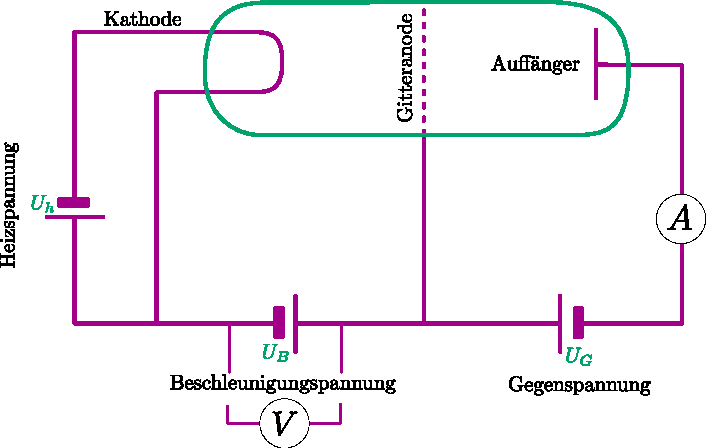
\includegraphics[width=\linewidth]{figures/frankhertzaufbau.pdf}
        \caption{Frank-Hertz-Versuch}
        \label{fig:frankhertzaufbau}
    \end{marginfigure}
    Der \highlight{Frank-Hertz-Versuch} ist ein Experiment, das die Quantisierung der Energiezustände von Atomen bestätigt. Der Versuchsaufbau besteht aus einer Vakuumröhre, in der Quecksilberdampf enthalten ist. Die Röhre wird durch eine Heizspannung erhitzt, sodass Quecksilberdampf entsteht. Elektronen, welche durch die aufgeheizte Glühkathode emittiert werden, werden durch eine Beschleunigungsspannung \highlight{$U_B$} beschleunigt. Die Elektronen werden auf die Quecksilberatome, die in der Quecksilberdampfatmosphäre herumschwirren, geschossen und regen diese an. Eine Gitteranode wird hinter der Glühkathode angelegt. 
    Nach dem Gitter wird eine weitere Anode, dem Auffänger, an diese eine konstante Spannung von \highlight{$U_A$} angelegt ist, aufgebaut. Diese Spannung ist so gepolt, sodass die Elektronen, die durch die Gitteranode treten, abgebremst werden. Ein empfindliches Strommessgerät ist an die Anode, dem Auffänger, angeschlossen. Die von diesem Gerät gemessene Stromstärke ist ein Maß für die Anzahl der Elektronen, die genügend Energie besitzen, um das Gegenfeld zwischen Gitter und Anode zu überwinden.
    \begin{marginfigure}
        \centering
        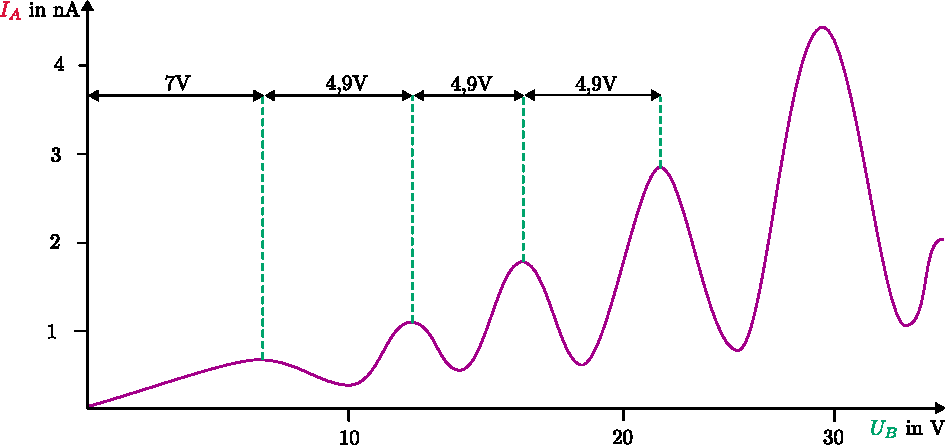
\includegraphics[width=\linewidth]{figures/frankhertzspannung.pdf}
        \caption{Der Anodenstrom \textcolor{crimson}{$I_A$} in Abhängigkeit von der Beschleunigungsspannung \highlight{$U_B$} zeigt Maxima in regelmäßigen Abständen. von 4.9V. Das erste Maximum liegt aufgrund der Wirkung von Kontaktspannungen erst bei ca. 7V.}
        \label{fig:frankhertzkurve}
    \end{marginfigure}
    \begin{beobachtung}
        \vspace{-1em}
        Wird die Beschleunigungsspannung \highlight{$U_B$} zwischen der Kathode und dem Gitter erhöht, so zeigt das Messgerät eine zu-nehmende Anodenstromstärke \textcolor{crimson}{$I_A$} an, die jedoch bei einer bestimmten Spannung wieder abfällt. 
    \end{beobachtung}
    \begin{deutung}
        \vspace{-1em}
        Die Elektronen werden durch das elektrische Feld zwischen Kathode und Gitter beschleunigt. Je größer die Beschleunigungsspannung \highlight{$U_B$} ist, desto größer ist auch die kinetische Enerrgie $E_{kin}$ der Elektronen. Mit zunehmender kinetischer Energie schaffen es immer mehr Elektronen, das Gegenfeld zwischen Gitter und Anode zu überwinden. Die Anodenstromstärke \textcolor{crimson}{$I_A$} steigt an, bis das erste relative Maximum erreicht ist. Der danach folgende Abfall der Stromstärke bedeutet, dass die Anzahl der zur Anode gelangenden Elektronen wieder sinkt. Es muss also ab dieser Beschleunigungsspannung Elektronen geben, die auf ihrem Weg von der Kathode zum Gitter Energie abgegeben haben. Ihre Energie reicht dann nicht mehr aus, um das Gegenfeld zu überwinden.
    \end{deutung}
    Elektronen müssen eine Mindestenergie besitzen, um die Quecksilberatome anzuregen: Auf ihrem Weg zum Gitter bzw. zur Anode treffen die Elektronen auf Quecksilberatome. Ist ihre Energie noch unterhalb der Mindestenergie, kommt es zu elastischen Stößen\sidenote{
        Bei einem \highlight{elastischen Stoß} bleiben sowohl die kinetische Energie $E_\text{kin}$ als auch der Impuls $\vec{p}$ erhalten:
        \[
        E_\text{kin, vor} = E_\text{kin, nach}, \quad \vec{p}_\text{vor} = \vec{p}_\text{nach}
        \]
        Es gibt keine Energieverluste durch Wärme, Verformung oder innere Prozesse. Ein Beispiel ist die Kollision zweier idealer Billardkugeln.} mit den Quecksilberatomen. Die Elektronen geben keine Energie an die Quecksilberatome ab. Besitzen die Elektronen jedoch eine Energie, die größer ist als diese Mindestenergie, so stoßen sie unelastisch\sidenote{Beim \highlight{inelastischen Stoß} bleibt zwar der Impuls erhalten,
        \[
        \vec{p}_\text{vor} = \vec{p}_\text{nach}
        \]
        %aber ein Teil der kinetischen Energie wird in andere Energieformen (z. B. Wärme, Verformung oder innere Anregung von Atomen/Molekülen) umgewandelt:
        \[
        E_\text{kin, nach} < E_\text{kin, vor}
        \]
        Ein vollständig inelastischer Stoß führt dazu, dass die Objekte nach der Kollision zusammenkleben.}. Sie geben Energie ab, und das Quecksilberatom geht in einen angeregten Zustand. 
        
        Es geht also ein Teil der kinetischen Energie der Elektronen in eine andere Energieform über. Nach einem unelastischen Stoß ist die verbleibende kinetische Energie der Elektronen nicht mehr genug, um das Gegenfeld zu überwinden, und die Stromstärke sinkt. 
        
        Wird die Beschleunigungsspannung weiter erhöht, so können die Elektronen nach einem unelastischen Stoß wieder Energie aufnehmen und die Anode erreichen. Die Stromstärke steigt wieder so lange, bis die Energie für einen zweiten unelastischen Stoß, d.h. einen Stoß mit Energieabgabe ausreicht. Dies entspricht dem zweiten Maximum in der Stromkurve.
        
        Bei weiterer Erhöhung der Beschleunigungsspannung wiederholen sich die Prozesse: Die Wegstrecken der Elektronen im elektrischen Feld zum Erreichen der Mindestenergie wird immer kürzer\sidenote{
            Dies ist auch der Grund, wieso die Stromstärke nur langsam nach dem Erreichen des Maximums sinkt, und nicht direkt $0$ wird. Es gibt Elektronen, die ohne Stöße mit den Quecksilberatomen an die Anode gelangen. Wird die Wegstrecke der Elektronen zur Anode immer kürzer, so sinkt die Wahrscheinlichkeit, dass die Elektronen auf ihrem Weg Energie abgeben.
            \begin{equation*}
                P_\mathrm{Stoss}\propto\frac{d}{\lambda}
            \end{equation*}
            Die Wahrscheinlichkeit $P_\mathrm{Stoss}$, dass ein Elektron mit einem Atom zusammenstößt hängt davon ab, wie weit $d$ das Elektron auf seinem Weg zur Anode zurücklegt.
            \begin{align*}
                E_{\mathrm{pot}} &= E_{\mathrm{kin}}\\
                E_{\mathrm{kin}} &= e\cdot U_B\\
                E_{\mathrm{kin}} &= \frac{1}{2}\cdot m_e\cdot v^2\\
                v &= \sqrt{\frac{2\cdot e\cdot U_B}{m_e}}\\
                \Rightarrow v&\propto\sqrt{U_B}\quad\land\quad d\propto v
            \end{align*}
            Da die Masse des Elektrons $m_e$ und die Elementarladung $e$ konstant sind, hängt die Geschwindigkeit $v$ der Elektronen nur von der Wurzel der Beschleunigungsspannung $U_B$ ab.
            Die Strecke $d$ hängt von der Geschwindigkeit $v$ der Elektronen ab. Die Geschwindigkeit ergibt sich aus der kinetischen Energie, die das Elektron durch die Spannung gewinnt.
            \begin{align*}
                P_\mathrm{Stoss}&\propto\frac{d}{\lambda}\propto\frac{\sqrt{U_B}}{\lambda}\quad\text{mit}\quad\lambda=\mathrm{konst.}\\
                \Rightarrow P_\mathrm{Stoss}&\propto\sqrt{U_B}
            \end{align*}
        }, die Elektronen stoßen entsprechend häufig mit den Quecksilberatomen und geben Energie ab. 
        
        Eine Auswertung des Diagramms zeigt, dass die Maxima der Stromstärke voneinander einen Abstand von $4.9\mathrm{eV}$ besitzen. Damit ergibt sich die Mindestenergie der Elektronen für einen unelastischen Stoß zu $4.9\mathrm{eV}$. Die Elektronen übertragen also bei einem unelastischen Stoß die Energie von $4.9\mathrm{eV}$.
        \begin{beobachtung}
            \vspace{-1em}
            Ist die kinetische Energie der Elektronen geringer als $4.9\mathrm{eV}$, so können die Quecksilberatome keine Energie bei einem Stoß aufnehmen. Die Elektronen stoßen elastisch mit den Atomen und behalten ihre kinetische Energie. Ist die Energie größer als die Mindestenergie von $4.9\mathrm{eV}$, kann ein Quecksilberatom einen Energiebetrag von $4.9\mathrm{eV}$ aufnehmen. Ein Quecksilberatom hat eine ca. $360.000$-mal größere Masse als ein Elektron.
        \end{beobachtung}
        Daraus folgt, dass es sich um eine innere Anregung des Atoms handeln muss, da die Energieaufnahme nicht zu einer Beschleinigung des Atoms führen kann. Es gibt also auch bei der Anregung durch Elektronenstoß eine \hyperref[def:quantenhafteabsorption]{quantenhafte Absorption}. Allerdings müssen die Elektronen, im Gegensatz zur Anregung mit Photonen, nicht einen genau den genau passenden Energiebetrag für die Anregung der Atome besitzen. Es reicht lediglich die Mindestenergie. Der Differenzbetrag bleibt dem Elektron als kinetische Energie.
        \begin{schlussfolgerung}
            \vspace{-1em}
            Der Frank-Hertz-Versuch bestätigt die Quantisier-ung der Energiezustände von Atomen. 

            Wird das Emissionsspektrum von Quecksilberatomen untersucht, so wird eine Linie der Wellenlänge $\lambda=253\mathrm{nm}$ im Bereich des ultravioletten Lichts beobachtet. Die Energie der zugehörigen Photonen beträgt:
            \begin{align*}
                E&=h\cdot f=h\cdot\frac{c}{\lambda}\\
                &=\frac{6.63\cdot10^{-34}\mathrm{Js}\cdot3.00\cdot10^8\frac{\mathrm{m}}{\mathrm{s}}}{253\cdot10^{-9}\mathrm{m}}\\
                E&=7.86\cdot10^{-19}\mathrm{J}=4.9\mathrm{eV}
            \end{align*}
        \end{schlussfolgerung}
        Quecksilberatome nehmen diesen Energiebetrag auf, gehen in einen angeregten Zustand über und emittieren Photonen dieser Energie bei dem anschließenden Übergang in den Grundzustand.



        \subsubsection{Atomspektren}
        \begin{marginfigure}
            \centering
            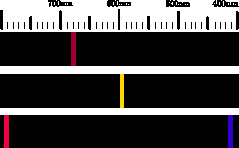
\includegraphics[width=\linewidth]{figures/akaliespektrallinien.pdf}
            \caption{Emissionsspektren der Alkalien Lithium (oben), Natrium (Mitte), und Kalium (unten)}
            \label{fig:akaliespektrallinien}
        \end{marginfigure}
        Atome emittieren Licht in Form von Spektrallinien. Diese Spektrallinien sind charakteristisch für jedes Element. Die \hyperref[fig:akaliespektrallinien]{Abbildung} zeigt die Linienspektren von chemisch sehr aktiven Alkalien. Anhand der vorkommenden farbigen Linien können das leuchtende Gas und damit seine atomaren Bestandteile \highlight{eindeutig} identifiziert werden. Die vorkommenden Linien sind für die Atome genauso einzigartig und charakteristisch, wie der Fingerabdruck eines Menschen.
        
        Bei manchen chemischen Elementen ist das von den Atomen emittierte Licht so charakteristisch, dass sie mithilfe einer \highlight{Flammenprobe} identifiziert werden können. Hierbei wird in eine Flamme die zu untersuchende Substanz gegeben. Die Flamme leuchtet dann in der Farbe, die aufgrund der additiven Farbmischung der Emissionslinien zustande kommt. 
        
        Das liegt daran, dass es durch die hohe Temperatur der Flamme zu unelastischen Stößen der Atome untereinander kommt, wodurch diese zur Lichtemission angeregt werden. Das resultierende Atomspektrum wird auch \highlight{Emissionsspektrum} genannt.
        \begin{marginfigure}
            \centering
            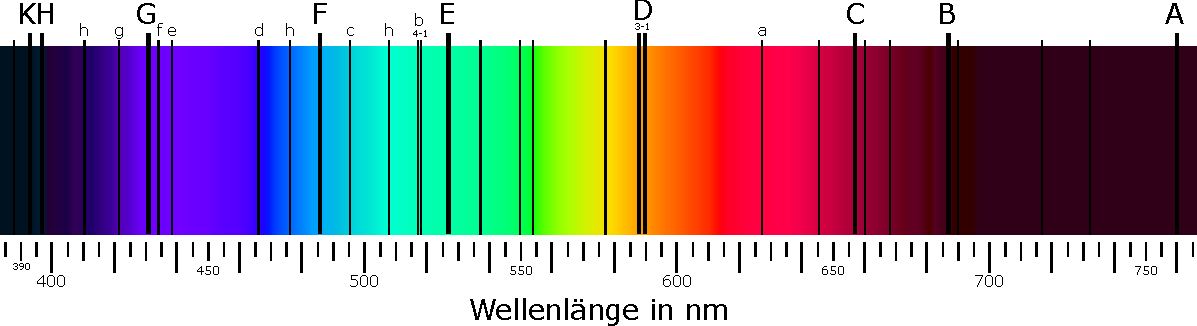
\includegraphics[width=\linewidth]{figures/frauenhoferlinien.pdf}
            \caption{Frauenhofer-Linien: Das Absorptionsspektrum des Sonnenlichts enthält aufgrund der Resonanzabsorption dunkle Linien.}
            \label{fig:frauenhoferlinien}
        \end{marginfigure}
        Auf der anderen Hand kann auch untersucht werden, welche Wellenlängen von Licht ein Atom absorbiert. Dazu wird das Licht einer Lichtquelle durch eine Dampfzelle mit dem zu untersuchenden Gas geleitet. Das Gas absorbiert dann genau die Wellenlängen, die den Energiedifferenzen der Niveaus entsprechen. Das resultierende Spektrum wird auch \highlight{Absorptionsspektrum} genannt.

        Beide Spektren sind charakteristisch für die Atome eines bestimmten Gases. Das Emissiosspektrum zeigt die Wellenlängen, die ein Stoff emittiert, während Absorptionslinien die Wellenlängen zeigt, die ein Stoff absorbiert. Die \hyperref[fig:frauenhoferlinien]{Frauenhofer-Linien} sind Absorptionslinien im Spektrum des Sonnenlichts. Sie entstehen durch die Resonanzabsorption von Atomen in der Sonnenatmosphäre. Die Atome absorbieren genau die Wellenlängen, die den Energiedifferenzen der Niveaus entsprechen. Damit sind die dunklen Linien im Spektrum des Sonnenlichts also charakteristisch für die Atome in der Sonnenatmosphäre\sidenote
        {
        Bei dem Aussenden der Sonnenstrahlung in Richtung Erde werden alle Atome wie z.B. Helium, Wasserstoff, Natrium, Eisen, etc. durchstrahlt. Diese Atome absorbieren dann genau die Wellenlängen, die ihrem Energiniveau entsprechen. Abschließend kommt es zur sogenannten \highlight{Reemission} des Lichts:
        \[\lambda_{\mathrm{absorbiert}}=\lambda_{\mathrm{reemittiert}}\]
        Das passiert, weil die Elektronen nach der Anregung des Atoms wieder auf ihren Grundzustand zurückfallen. Dabei wird die Energie in derselben Wellenlänge wieder abgegeben. Dies passiert \highlight{Isotrop}, also in alle Richtungen, weswegen im Endeffekt weniger dieser Wellenlängen in Richtung Erde gelangen. Die dunklen Linien im Spektrum des Sonnenlichts sind also charakteristisch für die Atome in der Sonnenatmosphäre.
        }.
        

        \subsubsection{Röntgenstrahlung}
        
        1895 entdeckte Conrad Willhelm Röntgen die nach ihm benannte \highlight{Röntgenstrahlung}. In einer Röntgenröhre werden von einer Glühkathode Elektronen emittiert, die in einem elektrischen Feld zwischen Kathode und Anode auf eine kinetische Energie von einigen zehntausend Elektronvolt beschleunigt werden. Diese treffena uf die Metallanode, wo aufgrund der starken Wechselwirkung der Elektronen mit den Metallatomen Röntgenstrahlung entsteht. Bei der Röntgenstrahlung handelt es sich um elektromagnetische Strahlung mit Wellenlängen der Größenordnung von $100\mathrm{pm}=10^{-12}\mathrm{m}$.
        \begin{marginfigure}
            \centering
            \incfig{roentgenroehre}
            \caption{Roentgenroehre.}
            \label{fig:roentgenroehre}
        \end{marginfigure}
        Die Röntgenstrahlung wird in zwei verschiedene Arten der Strahlung aufgeteilt:
        \begin{marginfigure}
            \centering
            \incfig{roentgenspektrum}
            \caption{Roentgenspektrum des Röntgenexperiments mit einer Kupferanode.}
            \label{fig:roentgenspektrum}
        \end{marginfigure}
        \begin{typ}
            \vspace{-1em}
            (Bremsstrahlung):
            \vspace{\baselineskip}

            \noindent Die Bremsstrahlung entsteht, wenn ein Elektron mit einer hohen kinetischen Energie in das elektrische Feld des Anodenmetals gelangt, und anschließend von dem positiv geladenen Atomkern abgelenkt wird. Dabei wird ein Photon emittiert, dessen Energie der kinetischen Energie des Elektrons entspricht. Die Energie des Photons ist also nicht quantisiert, sondern kann beliebige Werte annehmen.
            Das Spektrum das durch die Bremsstrahlung entsteht, ist kontinuierlich, da der Bremsprozess Sutfenweise abläuft, das heißt, dass Elektronen mit hoher Ladung graduell abgebremst werden, und somit ein kontinuierliches Spektrum emittieren.
        \end{typ}
        Die Bremsstrahlung wird hauptsächlich als Röntgenstrahlung in der Medizin für z.B. Tumorbehandlung eingesetzt\sidenote{Die Wellenlänge $\lambda_{\mathbf{min}}$ ist dort am kleinsten, wo die Energie $E$ am größten ist, da:
            \begin{equation*}
                \lambda_{\mathbf{min}}=\frac{h\cdot c}{E}
            \end{equation*}
            Und die Energie $E$ ist dort am größten, wo die Wellenlänge $\lambda_{\mathbf{min}}$ am kleinsten ist, da:
            \begin{equation*}
                E=\frac{h\cdot c}{\lambda_{\mathbf{min}}}
            \end{equation*}
        }.
        \begin{typ}
            \vspace{-1em}
            (Charakterisitsche Strahlung):
            \vspace{\baselineskip}

            \noindent Die charakteristische Strahlung entsteht, wenn ein beschleunigtes Elektron genug Energie hat, um die Bindungsenergie der Elektronen in der Atomhülle zu überwinden. Das Elektron wird aus der Atomhülle herausgeschlagen, und ein Elektron aus einer höheren Schale fällt in die entstandene Lücke. Dabei wird ein Photon emittiert, dass von dem Anodenmetall abhängig ist. Es kommt zu sogenannten "Peaks" im Spektrum, die charakteristisch für das Anodenmetall sind, da jedes Element sein eigenes Spektrum bestitzt.
        \end{typ}
        Die charakteristische Strahlung wird vor allem in zum Beispiel der Röntgenfluoreszenzanalyse (XRF) eingesetzt, um die Zusammensetzung von Materialien zu bestimmen. Die charakteristische Strahlung ist also einzigartig für jedes Element, und kann zur Identifikation von Materialien genutzt werden.
        
\end{document}